\section{\FullMethodName{}}
\label{sec:method}


Figure~\ref{fig:overview} summarizes our recipe for enabling fast and stable online RL from pretrained VLA models with \MethodName{}. The core idea is to maximally utilize the pretrained VLA to improve the efficiency of the RL training process. Training the entire VLA with online RL could be too compute- and sample-inefficient to produce an improved policy in just a few hours. Instead, we use the frozen VLA to provide the RL state representation, to supply reference actions and to guide exploration toward actions close to its own predictions, while still using a small actor and critic network.
We first adapt the VLA on a small amount of task-specific demonstration data, both to improve its initial task policy and to expose an RL token for downstream RL.
We then freeze the VLA and train lightweight off-policy actor and critic networks online, conditioning on both the RL token representation and the VLA's reference actions,
%%SL.3.16: try to avoid jargon, replace "chunked action interface" with something more self explanatory
%%KK.3.16: remove chunked action
and regularize the learned policy to stay close to the VLA model.
%%SL.3.16: Again, too much jargon -- unclear what "VLA prior" means (VLA is not a prior, it's a model that outputs actions). Can we rephrase in a more self-explanatory way?
%%KK.3.16: remove VLA prior - might need to write as VLA predicted action distribution
Our method turns online RL into local refinement of promising behaviors rather than unconstrained search. This design gives the online RL method the efficiency of a small actor-critic algorithm, while retaining the representation and behaviors of the pretrained VLA model. 

 
%%SL.2.15: Organizationally, I think the methods section is a bit disjointed right now. There are a number of exciting things in the method, but they are presented as a bit of a laundry list. I wonder if we can unify these things around a common theme: how do we leverage the VLA to enable the fastest, most efficient, and most stable real-world RL? Everything kind of contributes to this: we train the VLA to haev a special RL readout token, use a small model that benefits from both the VLA features and the VLA actions, and is constrained to explore behaviors that are close to those of the original VLA, such that the VLA also guides exploration...

% =========================================================
\subsection{Adapting the VLA to expose an RL interface}
\label{sec:rl_head}
%=========================================================

\begin{figure}

\includegraphics[width=0.5\textwidth]{figs/architecture.pdf}
    \captionof{figure}{\textbf{Details on RL token extraction.} \MethodName{} adds an encoder-decoder transformer to a pretrained VLA. It produces a compressed embedding of the VLA representation (the RL token). This representation then enables data and parameter efficient fine-tuning during online RL.}
    \label{fig:token}
\end{figure}

Sample-efficient online RL depends critically on the choice of state representation. Applying RL directly to the full VLA model is a poor match for rapid real-world adaptation: the representation is high-dimensional, and online updates to the billion-parameter model are both computationally expensive and sample-inefficient. At the same time, we would like to utilize the representation already contained inside a VLA after pretraining, since it was trained on large-scale web and robotic data and already contains information useful for generating actions for many tasks. However, it is generally not obvious which features from a transformer-based VLA make up a good representation for online RL and the embeddings in each transformer layer are high-dimensional. Our goal therefore is to compress the VLA representation into a compact embedding for RL that preserves task-relevant  information while remaining small enough for lightweight online actor-critic learning.


We achieve this by adding an \emph{RL token} (Fig.~\ref{fig:token}): a learned readout embedding that summarizes the VLA's knowledge into a small vector serving as the RL state.
Concretely, we obtain the RL token from a small additional transformer that we add to the pretrained VLA. We train this transformer in an encoder-decoder \citep{sutskever2014sequence} fashion, with the last input to the encoder being the RL token. Because the representation for the RL token must retain enough information to enable the decoder to reconstruct the inputs, it acts as a bottleneck.
Let $\mathbf{z} = f(s,\ell;\theta_{\text{vla}})$ denote the final-layer token embeddings produced by the pretrained VLA for state $s$ and language instruction $\ell$. The embeddings $\mathbf{z}$ decompose into $\mathbf{z}_{1:M} = \{\mathbf{z}_1,\dots,\mathbf{z}_M\}$, where each $\mathbf{z}_i$ corresponds to the embedding for one input token. 
We append a learned embedding $\mathbf{e}_\texttt{rl} = \mathbf{e}_\phi(\texttt{<rl>})$ to the sequence and process the augmented sequence with a lightweight encoder transformer $g_\phi$. The encoder output at the special-token position, denoted as $\mathbf{z}_{\text{rl}}$, is our RL token\footnote{In our experiments each task has a fixed language instruction, so we drop language embeddings in this step; the construction applies to all VLA embeddings in general.}
\begin{equation}
  \mathbf{z}_{\text{rl}} \;=\; g_\phi\!\bigl([\mathbf{z}_{1:M},\;\mathbf{e}_\texttt{rl}]\bigr)_{M+1}\,.
  \label{eq:readout}
\end{equation}
A decoder transformer~$d_\phi$ with a linear output projection $h_\phi$ is then trained to autoregressively reconstruct the original embeddings from $\mathbf{z}_{\text{rl}}$. Let $\bar{\mathbf{z}}_i = \mathrm{sg}(\mathbf{z}_i)$ denote the stop-gradient operation applied to VLA embeddings, then the autoregressive reconstruction objective on the demonstrations~$\mathcal{D}$ is given as:
\begin{equation}
  \mathcal{L}_{\text{ro}} = \mathbb{E}_{\mathcal{D}}\!\Bigl[\,
    \sum_{i=1}^{M}
      \bigl\lVert h_\phi\bigl(d_\phi([\mathbf{z}_{\text{rl}},\,\bar{\mathbf{z}}_{1:i-1}])\bigr)_{\!i}
        - \bar{\mathbf{z}}_i \bigr\rVert^2
  \,\Bigr].
  \label{eq:recon}
\end{equation}

We train the parameters~$\phi$ on a small task-specific demonstration dataset with the VLA considered frozen with respect to $\mathcal{L}_{\text{ro}}$, and (optionally) combine it with supervised fine-tuning of the VLA $(\theta_{\text{vla}})$. Afterwards, both $\theta_{\text{vla}}$ and $\phi$ are frozen, and online RL operates on the RL token representation $\mathbf{z}_{\text{rl}}$.

% =========================================================


\subsection{Online RL to refine VLA action chunks}
\label{sec:chunk_rl}
% =========================================================

After the initial adaptation stage we freeze both the VLA and the RL token representation. We then train lightweight actor ($\pi_\theta$) and critic ($Q_{\psi}$) networks online. Their inputs $x$ combine the RL token with any additional information useful to enable closed-loop control (e.g. the proprioceptive state of the robot). The critic model estimates the value of the state and action: $Q_{\psi}(\mathbf{x},\mathbf{a}_{1:C})\in \mathbb{R}$. Notably, rather than generating actions from scratch, the RL actor $\pi_\theta(\cdot | \mathbf{x}, \tilde{\mathbf{a}}_{1:C})$ is trained to refine action sequences $\tilde{\mathbf{a}}_{1:C}$ (referred to as action chunks) proposed by the VLA. 

\textbf{Training the critic.}  Our critic $Q_\psi( \mathbf{x},\mathbf{a}_{1:C})$ takes as input the state and the action chunk $\mathbf{a}_{1:C}$. We train the critic with standard off-policy temporal-difference learning on action chunk transitions sampled from the replay buffer $\mathcal{B}$:
\begin{equation}
\begin{aligned}
\mathcal{L}_Q&=\mathbb{E}_{(\mathbf{x}, \mathbf{a}_{1:C}, \mathbf{x}') \sim \mathcal{B}}
\Big[\big(\hat{Q}-Q_\psi(\mathbf{x}, \mathbf{a}_{1:C})
\big)^2\Big], \\
\hat{Q}&=\sum_{t'=1}^{C} \gamma^{t'-1} r_{t'}+\gamma^C\mathbb{E}_{\mathbf{a}' \sim \pi_\theta}
\Big[Q_{\psi'}(\mathbf{x}', \mathbf{a}')\Big].
\end{aligned}
\label{eq:critic_loss}
\end{equation}
where the input state is $\mathbf{x} =(\mathbf{z}_\text{rl}, \mathbf{s}^\text{p})$, and $\mathbf{s}^\text{p}$ denotes the proprioceptive state information, $\mathbf{z}_\text{rl}(\mathbf{s})$ denotes the RL token extracted for state $\mathbf{s}$; $\mathbf{x}'$ denotes the next input state; $\mathbf{a}' \sim \pi_\theta$ denotes taking a sample from the RL policy.  In practice, we follow TD3 \citep{fujimoto2018td3} and $\psi'$ are the parameters of the target network.


\textbf{Training the RL Policy.}
Our actor network $\pi_\theta(\cdot| \mathbf{x},\tilde{\mathbf{a}}_{1:C})$ produces a Gaussian action distribution over action chunks. It takes in the input state  \emph{and} a reference action chunk $\tilde{\mathbf{a}}_{1:C}$, and produces the action distribution: 
\begin{equation}
\pi_\theta\bigl(\mathbf{a}_{1:C} \mid \mathbf{x}, \tilde{\mathbf{a}}_{1:C}\bigr)
  =
  \mathcal{N}\Bigl(
    \mu_\theta\bigl(\mathbf{x}, \tilde{\mathbf{a}}_{1:C} \bigr),
    \sigma^2 \mathbf{I}
  \Bigr),
  \label{eq:policy}
\end{equation}
where, as before, $\mathbf{x} =(\mathbf{z}_\text{rl}, \mathbf{s}^\text{p})$.
Conditioning on $\tilde{\mathbf{a}}$ exposes the actor directly to the VLA’s predicted actions, so that online RL refines a strong initial proposal rather than learning from scratch. 
% Tobi: removed the below as it seems duplicated and the first part is more related work than something we want in methods?
%Unlike residual-policy parameterizations~\citep{TODO ResiP}, this design does not confine the actor to a hand-tuned residual scale, and therefore still allows free exploration of the action space when needed. 
A second benefit is that the sampled reference chunk preserves mode information from the VLA’s multimodal action distribution, which would otherwise be difficult for a unimodal Gaussian actor to recover~\cite{fql_park2025}.
We further stabilize learning by regularizing its action toward the reference action. Concretely, we optimize the actor to maximize critic value while staying close to the VLA reference chunk $\tilde{\mathbf{a}}$, similar in spirit to KL-regularized RL methods (see e.g.~\citep{peng2020learning,PetersREPS,Abdolmaleki2018MaximumAP,Dayan1997UsingEM,levine2018reinforcementlearningcontrolprobabilistic}). This effectively turns online RL into local action editing around the VLA generated action distribution, rather than an unconstrained search over high-dimensional action chunks. The objective for learning the RL policy is given as
\begin{equation}
\begin{aligned}
\mathcal{L}_{\pi}(\theta)
&=
\mathbb{E}_{\substack{\mathbf{s} \sim \mathcal{B} \\
\mathbf{a}_{1:C} \sim \pi_\theta}}
\left[
-\,Q_\psi(\mathbf{x}, \mathbf{a}_{1:C})
+\beta \left\|\mathbf{a}_{1:C}-\tilde{\mathbf{a}}_{1:C}\right\|_2^2
\right], \\
\qquad
& \qquad \tilde{\mathbf{a}}_{1:C}\sim\pi_{\mathrm{vla}}(\cdot\mid\mathbf{s}, \ell),
\end{aligned}
\label{eq:actor_loss}
\end{equation}
where the coefficient $\beta$ controls how strongly the actor is regularized towards the sampled VLA action. 

\textbf{Reference action dropout.} A practical failure mode of reference-action conditioning is that the actor may simply copy $\tilde{\mathbf{a}}$ instead of learning to improve it. This is especially likely before the critic becomes informative, since both conditioning on $\tilde{\mathbf{a}}$ and regularizing towards it encourage the actor to remain close to the VLA proposal. To prevent this, we apply \emph{reference action dropout}: for a random subset of transitions in each training batch, we replace the reference chunk with zeros before passing it to the actor. This forces the actor to maintain an independent action-generation pathway, while still allowing it to exploit the VLA action distribution whenever the reference chunk is present. In practice, once the critic provides useful signal, the actor naturally learns to deviate from the reference whenever doing so increases predicted value.


% =========================================================
% Algorithm box
% =========================================================
\begin{algorithm}[t]
\caption{\MethodName{}}
\label{alg:main}
\begin{algorithmic}[1]
\REQUIRE \textcolor{gray}{\textit{Frozen VLA backbone $f_{\theta_\text{vla}}$ and VLA action distribution $\pi_{\text{vla}}$;
demo data $\mathcal{D}$, chunk length $C$, replay buffer $\mathcal{B}$,
warmup steps $N_{\text{warm}}$, ratio $G$, VLA fine-tuning weight $\alpha$, policy constraint $\beta$.}} 
\vspace{2pt}

\STATE \textbf{Train RL token and (optionally) fine-tune the VLA}
\STATE Train $\phi$ using $\mathbf{z}_i=f_i(\mathbf{s}, \ell, \theta_\text{vla})$, $\mathbf{z}_{\text{rl}} = g_\phi([\mathbf{z}_{1:M}, \mathbf{e}_\text{rl}])_{M+1}$, and $\theta_\text{vla}$ (only if $\alpha > 0$).
\[
\mathcal{L}_{\text{ro}}(\phi) = \mathbb{E}_{\mathcal{D}}\!\Bigl[\,
    \sum_{i=1}^{M}
      \bigl\lVert h_\phi\bigl(d_\phi([\mathbf{z}_{\text{rl}},\,\bar{\mathbf{z}}_{1:i-1}])\bigr)_{\!i}
        - \bar{\mathbf{z}}_i \bigr\rVert^2
  \,\Bigr].
\]
\STATE 
\[
\phi, \theta_{\text{vla}} = \arg \min_{\phi, \theta_{\text{vla}}} \mathcal{L}_{\text{ro}}(\phi) + \alpha \mathcal{L}_{\text{vla}}(\theta_\text{vla})
\]
\vspace{2pt}

\STATE \textbf{Train RL actor and critic}
\STATE Initialize critic $Q_\psi$ and RL Policy $\pi_\theta$.
\FOR{environment steps $t=0,C,2C\dots$ }
  \STATE Sample VLA reference chunk $\tilde{\mathbf{a}}_{t:t+C-1}\sim \pi_{\text{vla}}(\mathbf{s}_t)$.
  \STATE Form RL state $\mathbf{x}_t = (\mathbf{z}_{\text{rl}}(\mathbf{s}_t), \mathbf{s}^p_t)$.
  \STATE $
\mathbf{a}_{t:t+C-1} \leftarrow
\begin{cases}
\mathbf{a}^{\text{human}} & \text{if intervention} \\
\tilde{\mathbf{a}}_{t:t+C-1}        & \text{if } t < N_{\text{warm}} \\
\sim \pi_\theta(\,\cdot \mid \mathbf{x}_t,\tilde{\mathbf{a}}\,) & \text{otherwise}
\end{cases}
$
  \STATE Execute $\mathbf{a}_{t:t+C-1}$ and observe $r_t$, $\mathbf{s}_{t+1}$, $\mathbf{s}^p_{t+1}$
\STATE $
\tilde{\mathbf{a}}_{t:t+C-1} \leftarrow \mathbf{a}^{\text{human}} \quad \text{if intervention} $
  \STATE Store transition in $\mathcal{B}$:\quad $\langle\mathbf{x}_t,\mathbf{a}_{t:t+C-1},\tilde{\mathbf{a}},r_t,\mathbf{x}_{t+1}\rangle$

  \FOR{$g=1,\dots,G$}
    \STATE Sample batch of data $\mathrm{b} \sim \mathcal{B}$.
    \STATE Compute target Q values
    \[
    \hat{Q} = \sum_{t'=1}^C \gamma^{t' - 1} r_{t'} + \gamma^{C} \mathbb{E}_{\mathbf{a}' \sim \pi_\theta} \big[ Q_{\psi'}(\mathbf{x}', \mathbf{a}') \big]
    \]
    \STATE Train Critic with TD backup (Eq. \eqref{eq:critic_loss})
    \[
    \mathcal{L}_Q(\psi) = \mathbb{E}_{\mathrm{b}} \Big[ 
    \big( \hat{Q} -   Q_\psi(\mathbf{x}, \mathbf{a}) \big)^2 \Big]
    \]
    \STATE Train Policy $\mathbf{a} \sim \pi_\theta(\cdot\mid \mathbf{s},\tilde{\mathbf{a}})$ (Eq. \eqref{eq:actor_loss})
    \[
      \mathcal{L}_{\pi}(\theta)=\mathbb{E}_\mathrm{b}\Bigl[
      -Q_\psi(\mathbf{x},\mathbf{a})
      +\beta\|\mathbf{a}-\tilde{\mathbf{a}}\|_2^2
      \Bigr] %\\ \text{where some of } \tilde{\mathbf{a}} \leftarrow 0
    \]
  \ENDFOR
\ENDFOR
\end{algorithmic}
\end{algorithm}

% =========================================================
\section{The Complete System}
\label{sec:system}
% 

\begin{figure*}[!htbp]
    \centering
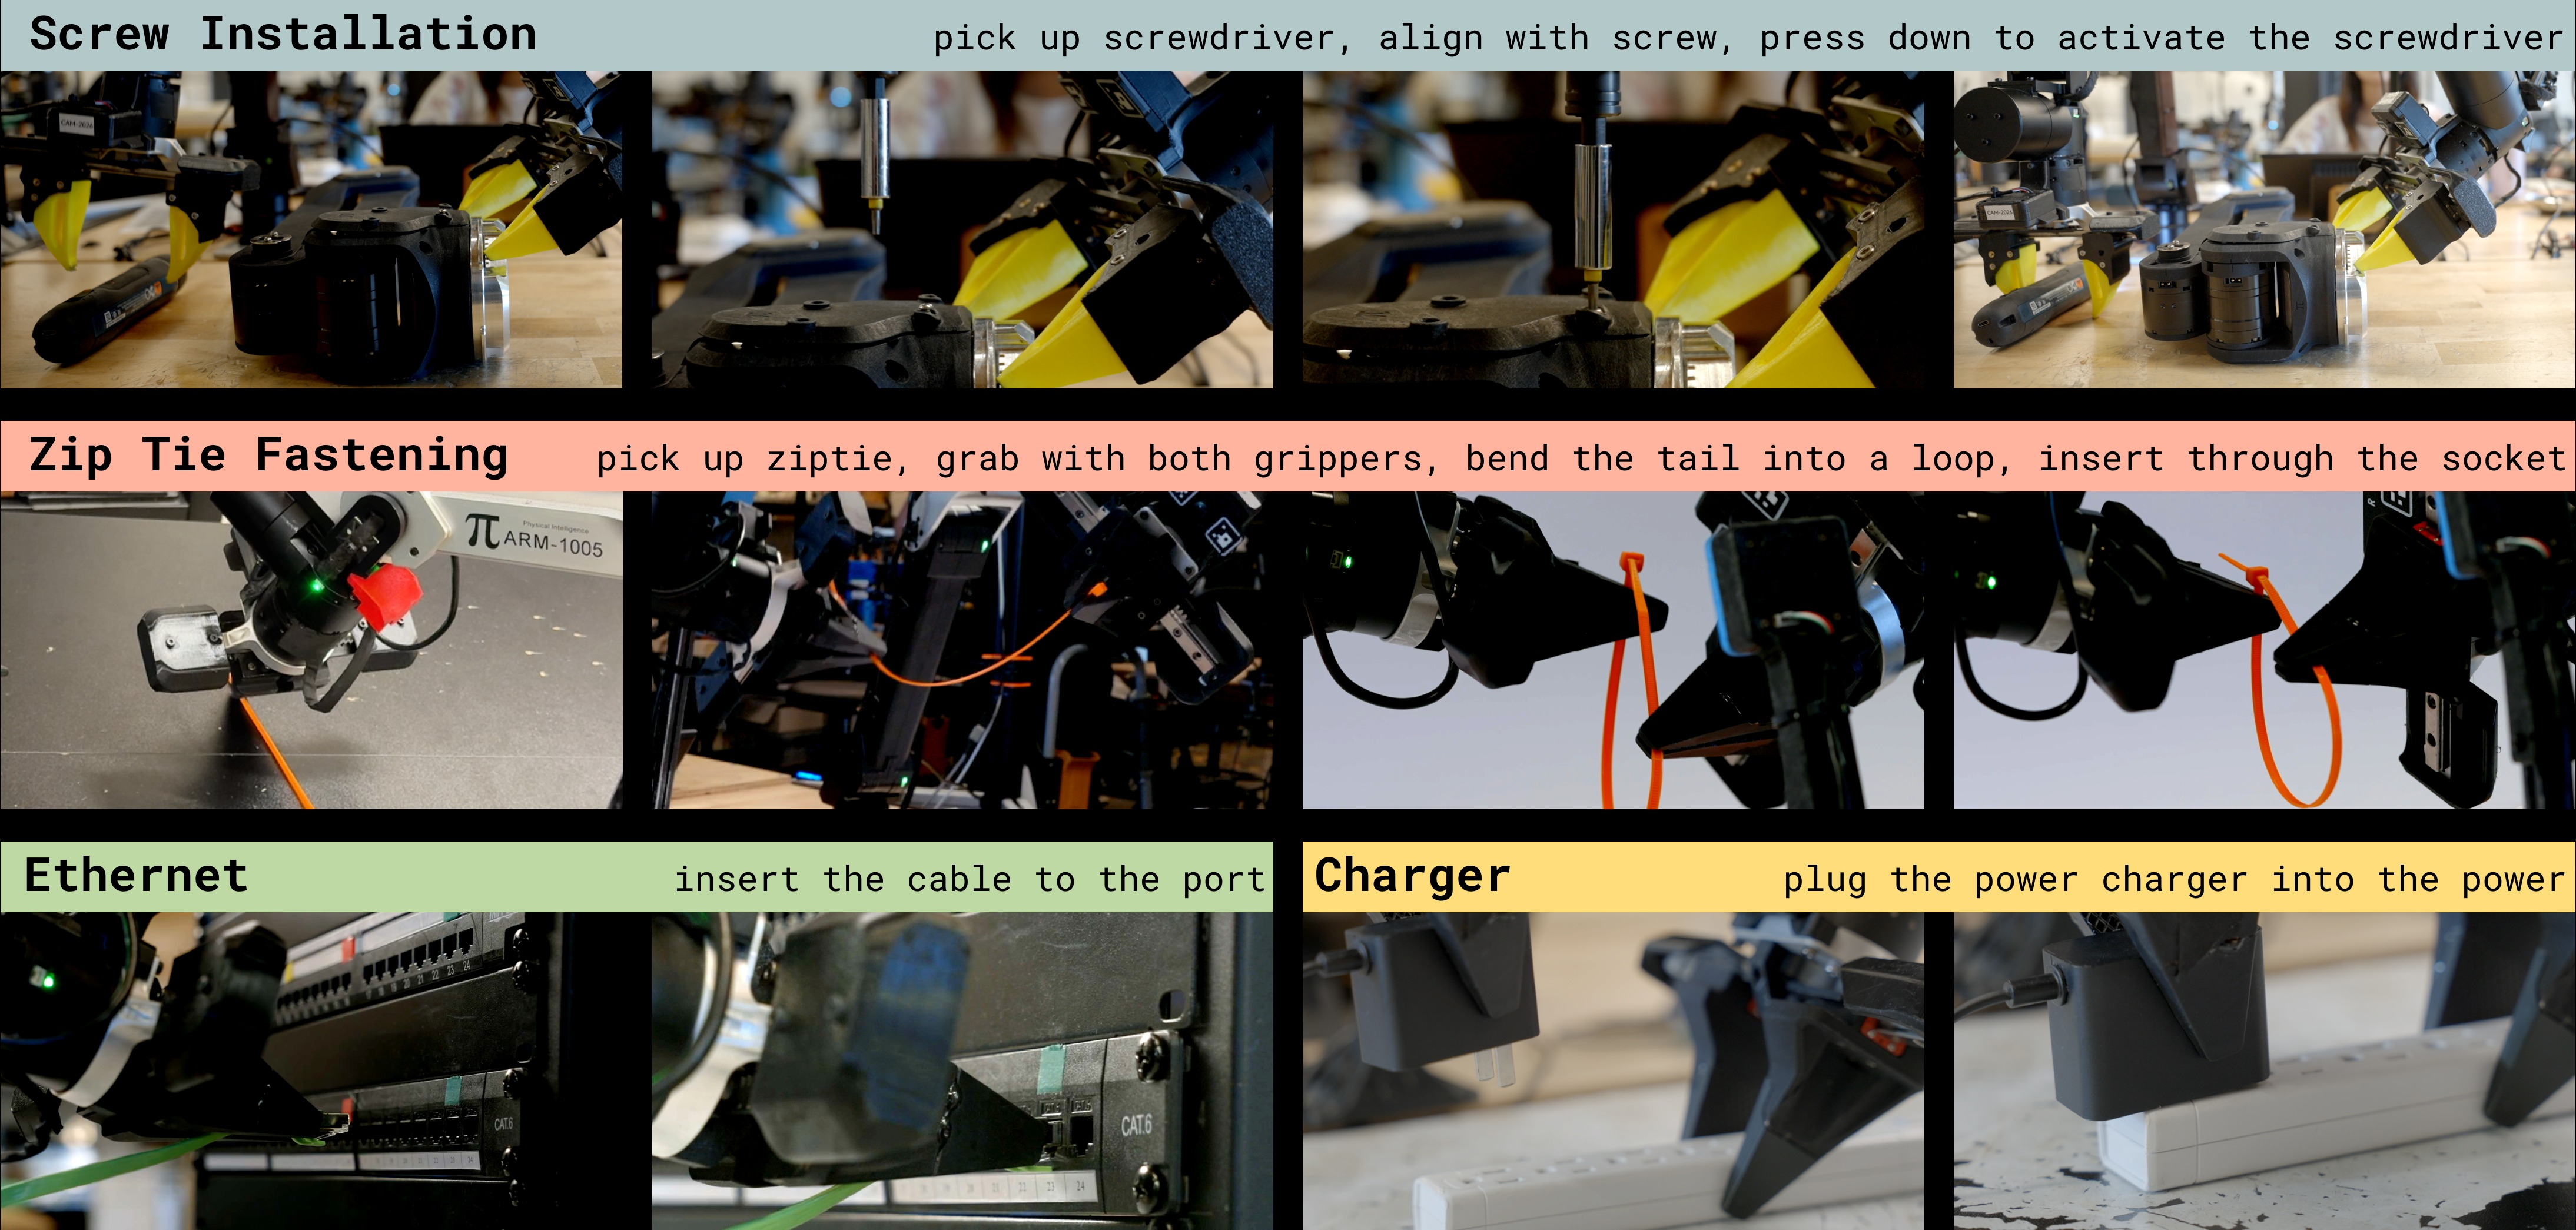
\includegraphics[width=1\linewidth]{figs/filmstrip.png}
%%SL.3.18: to fix the text in the figure:
% screwdriver installation: pick up screwdriver, align with screwn, push down to activate screwdriver
% zip tie fastening: pick up zip tie, grasp with both grippers, bend into a loop, insert into the socket
% Ethernet cable: insert the cable into the port
% Charger: plug the charger into the power strip
%%KK.3.18: done
    \caption{\textbf{The tasks in our experiments}: each task contains a critical phase that requires high precision: (top) using a screwdriver to install a screw, (middle) fastening a zip tie, (bottom) plugging in an Ethernet cable and plugging in a charger.}
    \label{fig:tasks}
\end{figure*}

Algorithm~\ref{alg:main} summarizes our full training loop. After an initial warmup stage to collect episodes with the base VLA policy, training alternates between collecting experience on the robot and performing off-policy actor-critic updates from replay. The replay buffer aggregates VLA warmup data, online RL rollouts, and optional human interventions. In addition, a human supervisor provides sparse success/failure labels. The steps are described in detail below. 

\textbf{Warmup.} After training the RL token representation (Sec.~\ref{sec:rl_head}), we pre-fill the replay buffer $\mathcal{B}$  by rolling out the VLA reference policy for $N_{\text{warm}}$ environment steps. This gives the critic an initial learning signal and ensures that online RL begins from competent VLA behavior.
%%SL.3.16: This seems a bit repetitive with the previous section, maybe we can shorten this so that we are not repeating ourselves as much?
%%KK.3.16: done.

\textbf{Rollout.} At each action chunk boundary during online collection, the frozen VLA produces a reference chunk $\tilde{\mathbf{a}}_{1:H}$ and the RL token module extracts $\mathbf{z}_{\text{rl}}$. The actor then outputs an action chunk $\mathbf{a}_{1:C} \sim \pi_\theta(\cdot \mid \mathbf{x}, \tilde{\mathbf{a}}_{1:C})$.
To accelerate learning of contact-rich or safety-critical behaviors, a human operator may optionally intervene by providing teleoperated commands $\mathbf{a}^{\text{h}}_{1:C}$ that overwrite the actor output for the duration of the intervention. When this occurs, the intervention replaces the VLA reference in the replay buffer. In all cases, each transition stored in $\mathcal{B}$ includes the executed action and the corresponding reference, enabling the actor to learn from both autonomous rollouts and human corrections.

%%SL.3.16: maybe we can use the notation introduced in the previous section to make this more precise and clearer?
%%SL.3.16: did we introduce the interventions before? this is a bit jarring without more context
%%KK.3.16: updated.

\textbf{Subsampling Action Chunks.} While the RL policy uses an action chunk length of $C$, we obtain observations for each intermediate step. We can thus increase data and improve learning efficiency by storing intermediate steps into the replay buffer. Concretely we pick a stride of $2$ and save transitions corresponding to $<\mathbf{x_0}, \mathbf{a_{0:C}}>, <\mathbf{x_2}, \mathbf{a_{2:C+2}}>, <\mathbf{x_4}, \mathbf{a_{4:C+4}}>, \dots$ to the replay buffer. Note that, due to the off-policy nature of our RL algorithm we can use all action chunks (including VLA-generated actions and human interventions).

\textbf{Update.} Policy updates are performed off-policy from the replay buffer according to Algorithm~\ref{alg:main}. To remain compute and time-efficient during training, we perform the rollouts and learning asynchronously. In practice, we perform two critic updates for each actor update, and begin learning shortly after the warmup phase. We use a high update-to-data ratio of $5$, which is essential in the low-data online regime.

\textbf{Targeted improvement of critical phases.}
%%SL.3.16: I would recommend using consistent terminology -- maybe we can call it critical phases throughout instead of interchangeably calling them bottlenecks?
%%KK.3.16: done
For practicality and efficiency of learning, we apply \MethodName{} to improve the critical phase of each task we consider -- corresponding to the most difficult sections which require high-precision -- and let the base VLA perform the easier parts of the task.
%%SL.3.16: avoid jargon like "precision-critical" etc
%%KK.3.16: done
Concretely, each episode starts by executing the base model. During data collection, a human operator can then choose at which point to hand the control from the base VLA to the RL policy. This is analogous to human intervention decisions in interactive imitation learning~\citep{kelly2019hgdaggerinteractiveimitationlearning}. Our system then applies RL to the chosen task segment, storing and training on transitions during this critical phase, until receiving a terminal signal from the human operator that indicates success or failure of the RL task. This concentrates data collection and credit assignment on the part of the behavior where online adaptation matters most. 
To enable autonomous execution at test time, we can conclude training with a final short fine-tuning phase of the VLA where we ask it to additionally predict when to hand over execution to the RL policy (using the human interventions as labels). We can then automatically trigger the switch of policies at test-time.

